\PassOptionsToPackage{table}{xcolor}  % as xcolor is automatically loaded by knitr
%\documentclass[jou,a4paper,draftfirst]{apa6}
%\documentclass[man,a4paper]{apa6}
\documentclass[man,a4paper,mask]{apa6}\usepackage[]{graphicx}\usepackage[]{color}
% maxwidth is the original width if it is less than linewidth
% otherwise use linewidth (to make sure the graphics do not exceed the margin)
\makeatletter
\def\maxwidth{ %
  \ifdim\Gin@nat@width>\linewidth
    \linewidth
  \else
    \Gin@nat@width
  \fi
}
\makeatother

\definecolor{fgcolor}{rgb}{0.345, 0.345, 0.345}
\newcommand{\hlnum}[1]{\textcolor[rgb]{0.686,0.059,0.569}{#1}}%
\newcommand{\hlstr}[1]{\textcolor[rgb]{0.192,0.494,0.8}{#1}}%
\newcommand{\hlcom}[1]{\textcolor[rgb]{0.678,0.584,0.686}{\textit{#1}}}%
\newcommand{\hlopt}[1]{\textcolor[rgb]{0,0,0}{#1}}%
\newcommand{\hlstd}[1]{\textcolor[rgb]{0.345,0.345,0.345}{#1}}%
\newcommand{\hlkwa}[1]{\textcolor[rgb]{0.161,0.373,0.58}{\textbf{#1}}}%
\newcommand{\hlkwb}[1]{\textcolor[rgb]{0.69,0.353,0.396}{#1}}%
\newcommand{\hlkwc}[1]{\textcolor[rgb]{0.333,0.667,0.333}{#1}}%
\newcommand{\hlkwd}[1]{\textcolor[rgb]{0.737,0.353,0.396}{\textbf{#1}}}%
\let\hlipl\hlkwb

\usepackage{framed}
\makeatletter
\newenvironment{kframe}{%
 \def\at@end@of@kframe{}%
 \ifinner\ifhmode%
  \def\at@end@of@kframe{\end{minipage}}%
  \begin{minipage}{\columnwidth}%
 \fi\fi%
 \def\FrameCommand##1{\hskip\@totalleftmargin \hskip-\fboxsep
 \colorbox{shadecolor}{##1}\hskip-\fboxsep
     % There is no \\@totalrightmargin, so:
     \hskip-\linewidth \hskip-\@totalleftmargin \hskip\columnwidth}%
 \MakeFramed {\advance\hsize-\width
   \@totalleftmargin\z@ \linewidth\hsize
   \@setminipage}}%
 {\par\unskip\endMakeFramed%
 \at@end@of@kframe}
\makeatother

\definecolor{shadecolor}{rgb}{.97, .97, .97}
\definecolor{messagecolor}{rgb}{0, 0, 0}
\definecolor{warningcolor}{rgb}{1, 0, 1}
\definecolor{errorcolor}{rgb}{1, 0, 0}
\newenvironment{knitrout}{}{} % an empty environment to be redefined in TeX

\usepackage{alltt}
%\documentclass[doc,a4paper]{apa6}

% this still does not get citations right; and table references are still broken.
% pandoc --default-image-extension=.pdf -s AMC-Database.tex --bibliography=Zotero.bib --csl=apa6.csl -o AMC-Database.docx

\usepackage[]{graphicx}
\usepackage[]{color}

%------------------------------------------------
% Track changes
\definecolor{colour_added}{rgb}{.1,.6,.1}
\definecolor{colour_removed}{rgb}{.8,.1,.1}
\definecolor{colour_moved}{rgb}{.1,.1,.8}
%For rendering the changes:
%\newcommand{\added}[1]{\textcolor{colour_added}{\bf{#1}}}
%\newcommand{\removed}[1]{\textcolor{colour_removed}{#1}}
%\newcommand{\moved}[1]{\textcolor{colour_moved}{#1}}

%For rendering the clean version:
\newcommand{\added}[1]{#1}
\newcommand{\removed}[1]{}
\newcommand{\moved}[1]{#1}

%------------------------------------------------

\usepackage{alltt}
\usepackage[american]{babel}
\usepackage[T1]{fontenc}
\usepackage[utf8]{inputenc}

\usepackage{amsmath}  	% for advanced math displays (e.g. definition of W in RSA)
\usepackage{amssymb}
\usepackage{booktabs}	% booktables
\usepackage{siunitx}		% align tables to decimal point: http://tex.stackexchange.com/questions/2746/aligning-numbers-by-decimal-points-in-table-columns


% rotating: sidewaytables. Declare that also sidewaystables should be moved to the end of the document.
\usepackage{rotating} 
% Bei Journal-Mode muss man DeclareDelayedFloatFlavor wegkommentieren	
% \DeclareDelayedFloatFlavor{sidewaystable}{table}
% \DeclareDelayedFloatFlavor{sidewaysfigure}{figure}

% For line breaks in tables
\usepackage{makecell}
\renewcommand\theadalign{tl}   % \makecells with line break should be top and left aligned
\usepackage{adjustbox} % for vertical alignment of cells

\usepackage{tabularx} 
\usepackage{tabulary} 
\usepackage{multirow}

% With that package, tables are single spaced
\usepackage{setspace}

\usepackage{listings}  % for inline code blocks
\lstset{
	basicstyle=\scriptsize\ttfamily, % the size of the fonts that are used for the code
	breaklines=true,  % sets automatic line breaking
	breakatwhitespace=true, % sets if automatic breaks should only happen at whitespace
	literate={ö}{{\"o}}1 % allow ö in Schönbrodt
}


\usepackage{url}	% links to headings
\usepackage{placeins} 	% flushes Figures before the next section starts
% use command \FloatBarrier

% To Do Notes
\usepackage[colorinlistoftodos, textsize=footnotesize]{todonotes}

%% APA-style citations
\usepackage{csquotes}
\usepackage[backend=biber,style=apa,hyperref=true,giveninits,uniquename=init]{biblatex}
\DeclareLanguageMapping{american}{american-apa}
\addbibresource{Zotero.bib}

% remove unwanted from .bib-file
\AtEveryBibitem{	
  \clearfield{day}
  \clearfield{month}
  \clearfield{labelday}
  \clearfield{labelmonth}
  \clearfield{number}
}

% Make specific adjustments to the Zotero-exported .bib-file
% The nested curly braces fuck up texCount (word count), so ignore it.
%TC:ignore
\DeclareSourcemap{ 
    \maps[datatype=bibtex]{
      \map{
	  % upper case after colon and ?
           \step[fieldsource=title,
                 match=\regexp{([:\?].?\s)(\w)},
                 replace=\regexp{$1\{\u$2\}}]
   	  % upper case after colon: Book titles
              \step[fieldsource=booktitle,
                    match=\regexp{(:.?\s)(\w)},
                    replace=\regexp{$1\{\u$2\}}]
	  % upper case for "R"
	         \step[fieldsource=title,
	               match=\regexp{(\s)R([\s\.:!?,])},
	               replace=\regexp{$1\{R\}$2}]
 	%  Hand coded {}'s from Zotero
     	         \step[fieldsource=title,
     	               match=\regexp{\\\{},
     	               replace=\regexp{\{}]
	        \step[fieldsource=title,
	              match=\regexp{\\\}},
	              replace=\regexp{\}}]   
     	         \step[fieldsource=author,
     	               match=\regexp{(Task\sForce\son\sStatistical\sInference)},
     	               replace=\regexp{\{$1\}}]
         \step[fieldsource=author,
           match=\regexp{(R\sCore\sTeam)},
           replace=\regexp{\{$1\}}]
       }
    }
}
%TC:endignore

\usepackage{hyperref} % should be loaded last as it redefines many Latex commands
\hypersetup{colorlinks, urlcolor=blue, citecolor=blue}

%========================================================================
%-----  Here starts the actual paper --------------------
%========================================================================

\title{Measuring Implicit Motives With the Picture Story Exercise (PSE): Databases of Expert-Coded German Stories, Pictures, and Updated Picture Norms}
\shorttitle{PSE text and picture database}

\twoauthors{Felix D. Schönbrodt}{Birk Hagemeyer\textsuperscript{a}, Veronika Brandstätter\textsuperscript{b}, Thomas Czikmantori\textsuperscript{b}, Peter Gröpel\textsuperscript{c}, Marie Hennecke\textsuperscript{b}, Laura S. F. Israel\textsuperscript{j}, Kevin Janson\textsuperscript{d}, Nina Kemper\textsuperscript{e}, Martin G. Köllner\textsuperscript{d}, Philipp Kopp\textsuperscript{f}, Andreas Mojzisch\textsuperscript{g}, Raphael Müller-Hotop\textsuperscript{f}, Johanna Prüfer\textsuperscript{h}, Markus Quirin\textsuperscript{f,k}, Bettina Scheidemann\textsuperscript{i}, Lena Schiestel\textsuperscript{j}, Stefan Schulz-Hardt\textsuperscript{h}, Larissa Sust\textsuperscript{j}, Caroline Zygar\textsuperscript{j}, Oliver C. Schultheiss\textsuperscript{d}
}
\leftheader{Schönbrodt et al.}
\twoaffiliations{Ludwig-Maximilians-University Munich}{\textsuperscript{a}Friedrich Schiller University Jena, \textsuperscript{b}University of Zurich, \textsuperscript{c}University of Vienna, \textsuperscript{d}Friedrich-Alexander University Erlangen-Nürnberg, \textsuperscript{e}Frankfurt University, \textsuperscript{f}Technical University of Munich, \textsuperscript{g}University of Hildesheim, \textsuperscript{h}University of Göttingen, \textsuperscript{i}Osnabrück University, \textsuperscript{j}Ludwig-Maximilians-University Munich, \textsuperscript{k}PFH Göttingen}
\date{\today}


% Schönbrodt, F. D., Hagemeyer, B., Brandstätter, V., Czikmantori, T., Gröpel, P., Hennecke, M., Janson, K., Kemper, N., Köllner, M., Kopp, P. M., Mojzisch, A., Müller-Hotop, R., Prüfer, J., Quirin, M., Scheidemann, B., Schiestel, L., Schulz-Hardt, S., Sust, L., Zygar, C., Schultheiss, O. C. (2018). Measuring Implicit Motives With the Picture Story Exercise (PSE): Databases of Expert-Coded German Stories, Pictures, and Updated Picture Norms.
% Schönbrodt, F. D., Hagemeyer, B., Brandstätter, V., Czikmantori, T., Gröpel, P., Hennecke, M., ..., Schultheiss, O. C. (2018). Measuring Implicit Motives With the Picture Story Exercise (PSE): Databases of Expert-Coded German Stories, Pictures, and Updated Picture Norms.


\authornote{
Felix D. Schönbrodt, Department of Psychology, Ludwig-Maximilians-Universität München, Germany. 
We embrace the values of openness and transparency in science (\url{http://www.researchtransparency.org/}). We therefore publish all data necessary to reproduce the reported results and provide reproducible scripts for all data analyses reported in this paper (\url{https://osf.io/dj8g9/} and \url{https://github.com/nicebread/PSE-Database}). 

Acknowledgements. We want to thank the following additional coders: Kira Bleck, Julia Boppel, Franziska Dombaj, Julia Fenkl, Miriam Frisch, Laura Götz, Franziska Herbig, Tina Höhlein, Sinja Hondong, Jennifer Jochheim, Tobias Kaiser, Eva Katzinger, Eva Margraf, Regina Oberwesterberger, Anna Ossmann, Dominik Özbe, Lea T. Riegl, Anna Röltgen, Anne Schnabel, Leonhard Schramm, Maria Schultheiss, Julia Tafelmaier, Lukas de Wall. We thank Claudio Lauper for transforming many stories into a sentence-wise format. We thank 14 LMU students of the 2018 PSE course who manually corrected 35,353 spelling errors in the database.

Parts of this research were funded by the German Research Foundation (SCHO 1334/1-1, Felix Schönbrodt; HA 6884/2-1, Birk Hagemeyer; SCHU 1210/3-1, Oliver Schultheiss; 254142454 / GRK 2070, Stefan Schulz-Hardt and Andreas Mojzisch) and the Swiss National Science Foundation (SNSF 100019\_156516, Marie Hennecke and Veronika Brandstätter).

Correspondence concerning this article should be addressed to Felix Schönbrodt, Leopoldstr. 13, 80802 München, Germany. Email: \href{mailto:felix.schoenbrodt@psy.lmu.de}{felix.schoenbrodt@psy.lmu.de}.
}

% Abstract: 250 words max, up to 5 keywords
\abstract{

% \todo[inline,color=blue!20!white]{
%
% This is an unedited manuscript accepted for publication in the European Journal of Personality. The manuscript will undergo copyediting, typesetting, and review of resulting proof before it is published in its final form.\newline
% \vspace{0.1cm}
%
% Please cite this preprint as: \newline
% Schönbrodt, F. D., Humberg, S., \& Nestler, S. (in press). Testing similarity effects with dyadic response surface analysis. European Journal of Personality. Retrieved from https://psyarxiv.com/8mpua/
%
% \vspace{0.1cm}
% }



We present two openly accessible databases related to the assessment of implicit motives using Picture Story Exercises (PSEs): (a) A database of 183,408 German sentences, nested in 26,389 stories provided by 4,570 participants, which have been coded by experts using Winter's (1994) coding system for the implicit affiliation/intimacy, achievement, and power motives, and (b) a database of 54 classic and new pictures which have been used as PSE stimuli. Updated picture norms are provided which can be used to select appropriate pictures for PSE applications.
Based on an analysis of the relations between raw motive scores, word count, and sentence count, we give recommendations on how to control motive scores for story length, and validate the recommendation with a meta-analysis on gender differences in the implicit affiliation motive that replicates existing findings.
Several potential applications of the databases are discussed, including (un)supervised machine learning of text content, psychometrics, and better reproducibility of PSE research.

%\todo[inline,color=blue!20!white]{Unpublished manuscript, draft version 0.2, 2018-07-10.}
}

\keywords{picture story exercise, implicit motives, database, pictures, manual coding, machine learning}
\IfFileExists{upquote.sty}{\usepackage{upquote}}{}
\begin{document}
\maketitle	%First line of text directly after \maketitle (no blank line)
Implicit motives are nonconscious motivational needs that orient, select, and energize behavior \parencite{mcclelland_human_1987}. A common approach to measuring implicit motives, such as affiliation, power, or achievement motives, is the Picture Story Exercise (PSE; \nptextcite{schultheiss_MeasuringImplicitMotives_2007,smith_motivation_1992}). The PSE is a modern, experimentally validated version of the classic Thematic Apperception Test \parencite{morgan_method_1935}. In this task, several ambiguous pictures are presented to participants who are asked to write an imaginative story in response to each picture. These stories are then coded by trained coders using empirically derived and validated content coding systems, which quantify the amount of motive imagery in each story. Motive-related imagery is used as an indicator for the strength of the implicit motive.

``Picture Story Exercise'' is a rather generic term as instructions, pictures, and coding systems can vary between applications. However, some standardization has taken place in recent years. For example, a standard set of six pictures has been suggested, which provides a roughly balanced motivational pull for each of the achievement, affiliation, and power motives \parencite{schultheiss_MeasuringImplicitMotives_2007}. However, the existence of such a standard picture set does not mean that other pictures should not be used: \textcite{schultheiss_MeasuringImplicitMotives_2007} recommended using other, specific picture sets if only one motive is assessed or one wants to predict behavior in a specific situational context based on pictures related to this context. Furthermore, multiple coding systems exist for several motives (for an overview, see \nptextcite{schultheiss_ImplicitMotives_2010}, or \nptextcite{smith_motivation_1992}). Many coding systems focus on one single motive, but one prominent exception is David Winter's (\citeyear{winter_ManualScoringMotive_1994}) \emph{Manual for scoring motive imagery in running text}. This integrated coding system allows to assess three implicit motives simultaneously \parencite{winter_MeasuringPersonalityDistance_1991}: the needs for achievement (\emph{ach}), power (\emph{pow}), and affiliation/intimacy (\emph{aff}).\footnote{Affiliation/intimacy is a fusion of originally separate coding systems for affiliation and intimacy. Here we use the abbreviation \emph{aff} for the combined affiliation/intimacy category.} It currently has been the most commonly employed system, and will be the focus of this publication.

The current paper has four goals: (1) To present a large database of stories that have been coded for implicit motives using the Winter coding system, (2) to provide a systematic database of 54 classic and new picture stimuli that have been used in PSEs, (3) to provide updated norms for picture pulls (i.e., the propensity of a picture to elicit a certain kind of motive image), and (4) to provide a recommended approach for how motive scores should be corrected for story length.

The text database can be used for several research topics, both within and beyond the field of implicit motives. These can include, for example, psychometric analyses of PSE measures, but also automated text analysis systems that replicate human codings in the Winter system. More generally, the text database can be used as training material for machine learning algorithms. The picture database allows to create specific stimulus sets for targeted PSE measurements. More details on potential applications are given below in the discussion.


\section{A Database of Coded PSE Stories}

Several labs contributed datasets for building a large database of coded PSE stories in German. The inclusion criteria were (a) the stories were coded using the Winter coding system, (b) all coders were trained by experts, had extensive coding experience, and achieved good convergence with training material coded by experts (such as ICC $\geq .85$, category agreement $\geq .85$), and (c) the stories were coded sentence-wise.
The included datasets come from a diverse range of studies, including lab and online administrations of the PSE tasks, differing numbers and types of pictures, and diverse samples. Some of the datasets come from published work \parencite{kollner_SocialBiopsychologyImplicit_2018,kollner_InfluenceImplicitMotives_2015,janson_InhibitedPowerMotivation_2018a,janson_ImplicitPowerMotive_2017,zygar_EinflussEmotionalerIntelligenz_2013,czikmantori_ExperienceIntrinsicMotivation_2018}, others are hitherto undocumented new or archival datasets. For a few of these archival datasets no person-level sample descriptives could be recovered. Table~\ref{tab:codebook} explains all variables of the database and their meaning, Table~\ref{tab:studies} provides an overview of all included primary raw data sources and some study-level descriptives.

\begin{table*}
\begin{threeparttable}
		\caption{Codebook for the PSE Story Database.}
		\label{tab:codebook}
		\footnotesize
		\begin{tabularx}{\textwidth}{llXX}
		\toprule
% latex table generated in R 3.5.2 by xtable 1.8-4 package
% Fri Sep 13 16:21:47 2019
Variable name & Data type & Comment & Values \\ 
  \hline
row\_id & numeric & Unique row id &  \\ 
  study\_id & factor & Identifier for the original study/data set &  \\ 
  coding\_lab & factor & Lab where the coders were trained & Munich, Erlangen, Osnabrueck, Trier \\ 
  scoring\_type & factor & Second sentence rule applied? & eachSentence, 2nd\_sentence\_rule \\ 
  participant\_id & factor & Unique person identifier &  \\ 
  gender & factor & Gender & m = male, f = female, NA = missing/other \\ 
  age & factor & Age category & $<$= 25, 25 $<$ age $<$= 35, 35 $<$ age $<$= 45, 45 $<$ age $<$= 55, age $>$ 55 \\ 
  USID & factor & Unique story identifier &  \\ 
  UTID & factor & Unique text identifier (each sentence is one 'text') &  \\ 
  pic\_id & factor & Unique picture identifier & See https://osf.io/pqckn/ \\ 
  pic\_position & numeric & Position of picture in PSE task. The number encodes the picture position of valid stories, and not the position of the presented picture (e.g., if the first story was empty, the second picture gets the position `1'). &  \\ 
  pic\_order & factor & Picture order in PSE task fixed for all participants, or variable? & fixed, variable \\ 
  unit & numeric & Sentence number within each story &  \\ 
  wc & numeric & Word count (at sentence level) &  \\ 
  sc & numeric & Sentence count (at story level) &  \\ 
  pow & numeric & Presence of power imagery & 0 (absent) or 1 (present) \\ 
  ach & numeric & Presence of achievement imagery & 0 (absent) or 1 (present) \\ 
  aff & numeric & Presence of affiliation/intimacy imagery & 0 (absent) or 1 (present) \\ 
  motclass & factor & Multiclass combination of aff, ach, and pow codings. All mixed codings are collapsed into the category 'mixed'. & none, ach, aff, pow, mixed \\ 
  motclassfull & factor & Multiclass combination of aff, ach, and pow codings with all possible combinations. & none, ach, aff, pow, achpow, affach, affpow, affachpow \\ 
  text & character & The text of the sentence. &  \\ 
   \hline

		\bottomrule
		\end{tabularx}
		\begin{tablenotes}[para,flushleft]
			{\small
			\vspace*{0.75em}
			\textit{Note.} In study \emph{MK3} there was a longer break between pictures 1--4 and 5--8.}
    \end{tablenotes}
\end{threeparttable}
\end{table*}







\begin{sidewaystable*}
\begin{threeparttable}
		\caption{Descriptives of Studies in the Database.}
		\label{tab:studies}
		\scriptsize
		\begin{tabularx}{\textwidth}{lrrrlllrrllll}
		\toprule


% latex table generated in R 3.5.2 by xtable 1.8-4 package
% Fri Sep 13 16:21:48 2019
Study ID & \# stories & n & \# pic & Scoring type & Coding lab & Pic. order & \% female & Date & Location & Admin. & Population \\ 
  \hline
BS & 814 & 144 &   6 & eachSentence & Osnabrueck & fixed & 84\% & 2014-2015 & de & CL & mostly students \\ 
  CZ & 987 & 141 &   7 & eachSentence & Munich & fixed & 73\% & 2013 & de & CO & students \\ 
  FS\_ErlSem & 287 &  41 &   7 & eachSentence & Munich & fixed & - & 2015 & de & H & students \\ 
  FS\_MOCO & 1009 & 144 &   8 & eachSentence & Munich & fixed & 79\% & 2013 & de & CO & mostly non-students \\ 
  FS\_newpic & 275 &  53 &  30 & eachSentence & Munich & variable & - & 2016 & de & CO & mostly non-students \\ 
  FS\_TSST & 578 &  97 &   6 & 2nd\_sentence\_rule & Munich & fixed & 53\% & 2011-2012 & de & CL & students \\ 
  JP & 3989 & 800 &   5 & eachSentence & Munich & variable & 50\% & 2016-2018 & de & CL \& CO & students \\ 
  KJ & 671 & 112 &   6 & eachSentence & Erlangen & variable & 58\% & 2015 & de & CL & mostly non-students \\ 
  LI & 1140 & 192 &   6 & eachSentence & Munich & fixed & 63\% & 2018-2019 & de & CO & mostly students \\ 
  LS & 3330 & 555 &   6 & eachSentence & Munich & fixed & 70\% & 2018-2019 & de & CO & students and non-students \\ 
  MK1 & 804 & 134 &   6 & eachSentence & Erlangen & variable & 59\% & 2015 & de & CL & N/A \\ 
  MK2 & 600 & 100 &   6 & eachSentence & Erlangen & variable & 50\% & 2013 & de & CL & N/A \\ 
  MK3 & 773 &  97 &   8 & eachSentence & Erlangen & variable & 45\% & 2015 & de & CL & N/A \\ 
  MOJ & 149 &  26 &   6 & eachSentence & Munich & fixed & 100\% & 2016 & de & CL & mostly students \\ 
  MQ & 486 &  81 &   6 & eachSentence & Munich & fixed & 88\% & 2012 & de & CO & students \\ 
  NK & 811 & 118 &   7 & 2nd\_sentence\_rule & Munich & fixed & 84\% & 2015 & de & CO & mostly students \\ 
  OCS\_Bp & 653 &  83 &   8 & eachSentence & Erlangen & variable & 51\% & 2013 & de & CL & mostly students \\ 
  OCS\_smofee6 & 984 & 164 &   6 & 2nd\_sentence\_rule & Erlangen & variable & 52\% & 2010 & de & CL & mostly students \\ 
  OCS\_smofee7 & 930 & 155 &   6 & 2nd\_sentence\_rule & Erlangen & variable & 51\% & 2011-2012 & de & CL & mostly students \\ 
  OCS\_smofee8 & 888 & 148 &   6 & eachSentence & Erlangen & variable & 48\% & 2012 & de & CL & mostly students \\ 
  OCS\_smofee9 & 893 & 149 &   6 & 2nd\_sentence\_rule & Erlangen & variable & 52\% & 2012 & de & CL & mostly students \\ 
  PMK & 1772 & 358 &   5 & eachSentence & Munich & fixed & 60\% & 2016-2017 & de & CO & students and non-students \\ 
  RMH & 698 & 176 &   4 & eachSentence & Munich & fixed & 45\% & 2016 & de & CL & students \\ 
  TC\_SNF6 & 676 & 136 &   5 & 2nd\_sentence\_rule & Trier & fixed & 72\% & 2015 & ch & CO & mostly non-students \\ 
  TC\_SNF7 & 1211 & 202 &   6 & 2nd\_sentence\_rule & Trier & fixed & 87\% & 2016 & ch & CO & mostly students \\ 
  TC\_TAI1 & 981 & 164 &   6 & 2nd\_sentence\_rule & Trier & fixed & 82\% & 2015 & ch & CO & students \\ 
   \hline


		\bottomrule
		\end{tabularx}
		\begin{tablenotes}[para,flushleft]
			{\small
			\vspace*{0.75em}
			\textit{Note.} $n$ = number of participants. Admin. = type of administration: CO = computer-written online, CL = computer-written in lab. de = Germany, ch = Switzerland. All PSEs were written in an individual setting, except study FS\_ErlSem which was in a group test setting.}
    \end{tablenotes}
\end{threeparttable}
\end{sidewaystable*}


\subsection{Winter's (1994) Coding System}
All stories were coded according to the Winter (\citeyear{winter_ManualScoringMotive_1994}) coding system, which defines rules for when to code a motive image for each motive category. A motive image is defined as ``an action (past, present, future, or hypothetical), a wish or concern, or some other internal state'' (p. 4) which is attributed to any character in a PSE story. Four to six specific content categories are defined for each motive (see Table~\ref{tab:wintercategories}). 


\begin{table*}
	\caption{Categories for Coding Motive Imagery \parencite{winter_MeasuringPersonalityDistance_1991,winter_ManualScoringMotive_1994}}
	\label{tab:wintercategories}
	\footnotesize
	\centering
	\begin{tabularx}{\textwidth}{lX}
		\toprule
        Motive & Categories \\
			\midrule
		  \adjustbox{valign=t}{\textbf{Affiliation/Intimacy}} & \makecell[l]{aff1: Positive, friendly, or intimate feelings towards others \\aff2: Negative feeling about separation \\aff3: Affiliative, companionate activities \\aff4: Friendly nurturant acts} \\

			\midrule
      \textbf{Achievement} & \makecell[l]{ach1: Adjectives that positively evaluate performance/outcomes \\ach2: Descriptions of goals/performances that suggest positive evaluation \\ach3: Winning or competing with others \\ach4: Negative feelings about failure, doing badly, lack of excellence \\ach5: Unique accomplishment} \\

			\midrule
      \textbf{Power} & \makecell[l]{pow1: Strong, forceful actions which inherently have an impact on other people \\pow2: Control or regulation \\pow3: Attempts to convince, persuade, influence, argue, make a point, etc. \\pow4: Giving help, support, or advice that is not explicitly solicited \\pow5: Impressing others, concern about fame, prestige, reputation \\pow6: Strong emotional reactions in one person to intentional actions of another person} \\
		\bottomrule
	\end{tabularx}
\end{table*}



The unit of coding is the sentence. Each sentence can be independently coded for the presence of any of the three motive categories \emph{aff}, \emph{ach}, or \emph{pow}. The manual defines an exception to this rule: If a certain motive has been coded (e.g., \emph{aff}), then another motive image is present (e.g., \emph{pow}) and then the first motive category \emph{aff} is present again in the same sentence, it can be coded twice in a sentence. The current database, however, does not incorporate such double codings of a motive in a single sentence and only codes the dichotomous presence (= 1) or absence (= 0) of a motive image for each sentence. This method of coding allows to combine the slightly different lab-specific coding conventions, and furthermore facilitates later use of the database for automatic text analyses.
Following from the combinations of the three motive categories, a sentence can belong to no category (\emph{null}), a single category (e.g., \emph{ach}), or multiple categories (e.g., \emph{achaff} or \emph{achaffpow}).

A second deviation from the manual concerns the ``2nd-sentence-rule''. This coding convention states that a motive of a certain category cannot be coded in two consecutive sentences. For example, if \emph{ach} imagery is present in three consecutive sentences, it is only coded in the first and the third sentence. However, the same motive can be coded in both of two consecutive sentences if the two categories are separated by codings for another motive. Several labs abandoned this 2nd-sentence rule, as it unnecessarily increases the frequency of the \emph{null} category and distorts analyses for psychometric models. The majority of all stories (73.2\%) was coded without applying the 2nd-sentence-rule. Hence, in these stories each sentence is coded independently of the codings of the previous sentence.

Finally, some of the stories of the included studies were coded by multiple coders. In some cases, differences were resolved via discussion and coders agreed on a final coding. In other cases, however, the diverging scores were averaged, which could lead to fractional scores, such as 0.5 \emph{aff}. As one main purpose of the database is to provide training data for automatic text analysis, which requires unambiguous assignments of sentences to categories, we decided to enter only distinct scores of 0 or 1. In cases where multiple experts coded the same stories and did not agree, we either relied on the coder who demonstrated the better performance, measured by agreement with expert-coded material, who had more experience in coding PSE stories, or, for consistency, used a coder who coded multiple included PSE datasets.

Stories were minimally preprocessed by automatically splitting them into sentences, converting all words to lowercase, and by removing trailing and leading whitespace. Furthermore we put in some effort to correct spelling errors. However, given the size of the database and that no fully automatic correction is possible, some typographical errors may remain in the stories. Table~\ref{tab:dathead} shows some rows of the dataset, and how sentences are coded (Note: Grammatical errors are from the original texts, as provided by participants.).


\begin{table*}
		\caption{Exemplary Sentences and Their Codes for Motive Imagery.}
		\label{tab:dathead}
		\rowcolors{2}{gray!15}{white}
		\footnotesize
		\begin{tabularx}{\textwidth}{XXrrrl}
		\toprule
		
% latex table generated in R 3.5.2 by xtable 1.8-4 package
% Fri Sep 13 16:21:48 2019
Text (original) & Text (translation) & ach & aff & pow & motclassfull \\ 
  \hline
der reporter im bild versucht sich einen eindruck vom leben der beschäftigten der schifffahrt in der vergangenheit zu machen. & The reporter in this picture is trying to get a sense of how ship employees lived in the past. &   0 &   0 &   0 & null \\ 
  als er erfährt, dass dieser kapitän bei einem unwetter über 100 leben gerettet hat, beginnt er aufgeregt der sache auf den grund zu gehen. & When he finds out that this captain saved more than 100 lives during a storm, he excitedly begins to investigate the matter. &   0 &   0 &   1 & pow \\ 
  immerhin könnte das die geschichte sein, auf die er seit langem wartet. & After all, this could be the story he has been waiting for for a long time. &   0 &   0 &   0 & null \\ 
  zwei freundinnen treffen sich um eine party vorzubereiten. & Two friends get together and prepare a party. &   0 &   1 &   0 & aff \\ 
  dazu sitzen auf der terasse in einem restaurant und sammeln ideen für ein motto. & For this purpose, they are sitting on the terrace of a restaurant collecting ideas for the party’s theme. &   0 &   1 &   0 & aff \\ 
  außerdem wollen kurz aufteilen wer welche aufgaben bei der vorbereitung übernimmt. & Besides, they want to divvy up what needs to be done in preparation. &   0 &   0 &   0 & null \\ 
  hinzu kommt ein weiterer freund, der die beiden erkannt hat. & Another friend, who has recognized them, joins. &   0 &   1 &   0 & aff \\ 
  er möchte kurz eine minute aufmerksamkeit der beiden haben um hallo zu sagen. & He wants to get the girls’ attention for a bit to say hello. &   0 &   1 &   0 & aff \\ 
  die beiden sind so vertieft in ihre arbeit, dass sie ihn gar nicht erst wahrnehmen. & Both girls are so absorbed in their work that they do not even notice him. &   0 &   0 &   0 & null \\ 
  da er scheinbar schon länger steht ist er bereits etwas genervt. & It looks like he has been standing there for a while now and he is already somewhat annoyed. &   0 &   0 &   0 & null \\ 
  wir befinden uns im zirkus rogalli. & We are at circus Rogalli. &   0 &   0 &   0 & null \\ 
  die zwei akrobaten im bild sind bekannt für ihre gefährlichen kunststücke am trapez. & The two acrobats in the picture are famous for their dangerous feats on the trapeze. &   1 &   0 &   1 & achpow \\ 
  mit ihrer neuen nummer gehen sie noch ein stück weiter. & They go one step further with their new stunt. &   1 &   0 &   0 & ach \\ 
   \hline

		\bottomrule
		\end{tabularx}
\end{table*}

\subsection{Descriptive Statistics}

The database combines coded PSE stories from 26 studies. Overall, 54 different pictures were used, although 30 of them (``newpic'') were just recently added and some of them have only very few coded stories (see Table~\ref{tab:norms}). Therefore all picture-related descriptive statistics below have been computed pictures that have at least 50 coded stories.

Overall, the database consists of 183,408 sentences coded with the Winter system, which are nested in 26,389 stories provided by 4,570 participants. Most participants wrote stories to 5 pictures (29.2\%) or 6 pictures (52.7\%) during their PSE task. The other studies had four, seven, or eight pictures. A story had on average 6.9 (\emph{SD} = 3.3) sentences and 92.3 (\emph{SD} = 35.6) words. These counts were roughly comparable for all pictures, ranging from an average sentence count of 5.1 for picture \emph{neymar \& marcelo} to 7.6 for \emph{sorrow}. The average word count was between 78 and 107, except for picture \emph{neymar \& marcelo} which had only 59 words on average.


Table~\ref{tab:motcat} shows the frequency of codings for each of the three motives. These proportions were only computed on studies that did not apply the 2nd-sentence-rule. Most sentences did not receive any motive category, and only a few sentences had simultaneously two or even all three motive categories.

% latex table generated in R 3.5.2 by xtable 1.8-4 package
% Fri Sep 13 16:21:48 2019
\begin{table}[ht]
\centering
\caption{Frequency of motive codes and their combinations.} 
\label{tab:motcat}
\begin{tabular}{ll}
  \hline
Motive category & Frequency \\ 
  \hline
null & 58.7\% \\ 
  aff & 13.9\% \\ 
  pow & 13.7\% \\ 
  ach & 9.3\% \\ 
  affpow & 2.3\% \\ 
  achpow & 1.6\% \\ 
  affach & 0.4\% \\ 
  affachpow & 0.2\% \\ 
   \hline
\end{tabular}
\end{table}



\subsection{The Relation of Story Length and Raw Motive Scores}

It has been shown that motive counts have a positive correlation with the length of the story, indicated by either word count or sentence count \parencite{pang_ContentCodingMethods_2010,schultheiss_MeasuringImplicitMotives_2007}. This phenomenon can have several causes: (A) To some extent, it follows from the structure of the coding system. As the unit of coding in the Winter system is the sentence, longer stories with more sentences can (potentially) accumulate more motive images. More specifically, the coding system as implemented in the current database (i.e., without multiple codes of a motive category in a single sentence) imposes an upper limit on codable motive images. For example, a story with four sentences cannot have more than four motive codings for each of the three motives, if the 2nd-sentence rule is not applied.
(B) A confounding with unrelated variables, such as verbal fluency, typing speed, creativity, or general vividness of fantasy can cause the relationship. From this perspective, persons who have more experience in typing on a computer keyboard have longer stories and are consequently ascribed stronger motives in the absence of a control for story length.
(C) The length of the story can also contain an actual signal related to implicit motives. Persons with a strong implicit motive are assumed to have a dense associative network which connects autobiographical experiences, situational cues, emotional experiences, and behavioral strategies around a motivational theme \parencite{schultheiss_reliability_2008,mcclelland_human_1987}. It is plausible that such a dense associative network makes it easier to generate rapidly available motive-related imagery, which results in more elaborate stories. From this perspective, an increased number of codings due to longer stories is a valid indicator of motive strength.

In practice, every PSE dataset probably features a mixture of all factors. The challenge is that motive researchers typically want to control for A and B, but not for C. But any attempt to control for one factor probably has unwanted side-effects on factors that contain a true signal (``overcontrolling''). Consequently, there is no easy solution to this problem. Typically two methods have been employed to deal with these confounds \parencite{schultheiss_MeasuringImplicitMotives_2007}: Either (linearly) residualizing motive scores for word count, or computing density scores (i.e., motive codings per 1000 words). Since the unit of coding is the sentence, however, both residuals and density scores could arguably be computed with sentence count instead of word count.\footnote{Given that the modeled outcome variable (i.e., raw motive codings) represents strictly non-negative count data, more specific regression approaches would be appropriate. The distributions of raw motive scores of all three motives follow very closely a negative binomial distribution, which suggests a corresponding generalized linear model for count data. However, the main focus of the current analysis is not the hypothesis test, and the residuals on person level from a Gaussian linear regression correlate $\geq .90$ with residuals from a negative binomial regression. Therefore, we focus on the traditionally applied Gaussian linear models and acknowledge the model misspecification, in order to increase the simplicity of practically applying the correction.}

For an empirical analysis of the word/sentence count and raw motive scores relations, we reduced the dataset to 3332 persons, nested in 17 studies which did not apply the 2nd-sentence rule and did not use pictures with too few stories. 
Table~\ref{tab:descCor} shows descriptive statistics and bivariate correlations between key variables. 
Traditionally, story length correction has been done on person level, by aggregating both the raw motive scores and the word counts across all picture stories of a person. 
Therefore, the correlations in Table~\ref{tab:descCor} also are on person level. 
As the number of pictures differed between included studies, the correlations were computed within study and then meta-analytically aggregated across studies. Means and \emph{SD}s, in contrast, were computed per picture story, as the number of pictures varies between studies. 


\begin{sidewaystable*}
%\begin{table*}
	\begin{threeparttable}
		\caption{Descriptive Statistics for Raw Motive Scores, Word Count, and Sentence Count per Picture Story, and Correlations on Person Level.}
		\label{tab:descCor}
		\footnotesize
		%\begin{tabular}{lrrlllllllllllllllll}
		\begin{tabularx}{\textwidth}{Xrrlllllllllllllllll}
		\toprule
% latex table generated in R 3.5.2 by xtable 1.8-4 package
% Fri Sep 13 16:21:49 2019
 & Mean & SD & (1) & (2) & (3) & (4) & (5) & (6) & (7) & (8) & (9) & (10) & (11) & (12) & (13) & (14) & (15) & (16) & (17) \\ 
  \hline
(1) Aff motive score & 1.13 & 0.73 & - & .87 & .90 & .73 & .68 & .22 & .06 & .09 & -.06 & -.05 & .24 & -.04 & .03 & -.03 & -.04 & .50 & .44 \\ 
  (2) Aff motive score, word count resid. & 0.00 & 3.08 &  & - & .93 & .91 & .80 & .06 & .06 & .04 & .05 & .01 & -.04 & -.05 & -.09 & -.06 & -.11 & .00 & .07 \\ 
  (3) Aff motive score, sentence count resid. & 0.00 & 3.22 &  &  & - & .82 & .87 & .10 & .04 & .11 & -.01 & .07 & .04 & -.09 & .04 & -.08 & .02 & .18 & .00 \\ 
  (4) Aff motive density (per 1000 words) & 12.95 & 7.57 &  &  &  & - & .84 & -.01 & .05 & .01 & .09 & .01 & -.13 & -.06 & -.13 & -.07 & -.13 & -.16 & -.05 \\ 
  (5) Aff motive density (per sentence) & 0.18 & 0.10 &  &  &  &  & - & -.01 & .01 & .07 & .02 & .18 & -.10 & -.10 & .02 & -.09 & .10 & -.04 & -.28 \\ 
  (6) Ach motive score & 0.78 & 0.51 &  &  &  &  &  & - & .94 & .96 & .80 & .76 & .21 & .02 & .08 & .03 & .01 & .34 & .29 \\ 
  (7) Ach motive score, word count resid. & 0.00 & 2.49 &  &  &  &  &  &  & - & .97 & .91 & .84 & .02 & .02 & .00 & .02 & -.03 & .00 & .05 \\ 
  (8) Ach motive score, sentence count resid. & 0.00 & 2.52 &  &  &  &  &  &  &  & - & .86 & .87 & .07 & .00 & .08 & .00 & .05 & .11 & .00 \\ 
  (9) Ach motive density (per 1000 words) & 9.18 & 6.06 &  &  &  &  &  &  &  &  & - & .89 & -.09 & .01 & -.05 & .01 & -.06 & -.21 & -.12 \\ 
  (10) Ach motive density (per sentence) & 0.12 & 0.08 &  &  &  &  &  &  &  &  &  & - & -.08 & -.03 & .05 & -.03 & .10 & -.12 & -.29 \\ 
  (11) Pow motive score & 1.23 & 0.90 &  &  &  &  &  &  &  &  &  &  & - & .84 & .88 & .81 & .75 & .56 & .48 \\ 
  (12) Pow motive score, word count resid. & 0.00 & 3.21 &  &  &  &  &  &  &  &  &  &  &  & - & .91 & .94 & .81 & .00 & .09 \\ 
  (13) Pow motive score, sentence count resid. & 0.00 & 3.37 &  &  &  &  &  &  &  &  &  &  &  &  & - & .86 & .91 & .21 & .00 \\ 
  (14) Pow motive density (per 1000 words) & 13.58 & 8.93 &  &  &  &  &  &  &  &  &  &  &  &  &  & - & .86 & .03 & .09 \\ 
  (15) Pow motive density (per sentence) & 0.19 & 0.13 &  &  &  &  &  &  &  &  &  &  &  &  &  &  & - & .11 & -.14 \\ 
  (16) Word count per story & 90.65 & 31.87 &  &  &  &  &  &  &  &  &  &  &  &  &  &  &  & - & .76 \\ 
  (17) Sentence count per story & 6.75 & 2.72 &  &  &  &  &  &  &  &  &  &  &  &  &  &  &  &  & - \\ 
   \hline

		\bottomrule
		\end{tabularx}
		\begin{tablenotes}[para,flushleft]
			{\small
			\vspace*{0.75em}
			\textit{Note.} Analyses in this table are based on 3332 persons, nested in 17 studies which did not apply the 2nd-sentence rule and did not use the new pictures. Mean and \emph{SD} are computed per picture story, as the number of pictures varies between studies. The correlations are computed within study on person level and then meta-analytically aggregated across studies.}
	      \end{tablenotes}
	  \end{threeparttable}
%\end{table*}
\end{sidewaystable*}


\subsubsection{The joint impact of sentence and word counts on overall motive scores}
Concerning potential indicators of story length, sentence count sets an upper limit of attainable motive codings in our database.\footnote{Again, this applies because we allowed a maximum of one coding per sentence per motive. In the original Winter coding system, multiple codings per motive are possible if two motive images are separated by another motive image within the same sentence.} But word count could have an incremental contribution, as longer sentences might have a higher chance of getting a motive coding. Therefore, we analyze the unique and common impact of both indicators of story length. Again, we performed the analyses on person level by aggregating raw motive scores, word counts, and sentence counts across all pictures stories of each person.

Furthermore, slopes for word and sentence count might vary between studies. To allow and account for such variations and the nested structure of the data set, we computed mixed effects models with sentence and word count as predictors, and random intercepts and slopes for the grouping variable \emph{study\_id}. In order to attain model convergence, we $z$-standardized sentence and word count and excluded covariances between random effects \parencite{bates_parsimonious_2015}. Finally, we explored the incremental contribution of squared sentence and word count. We added squared predictors as fixed effects, but did not add random slopes for the squared terms due to convergence problems.

Table~\ref{tab:mlmtab} summarises the explained variance of the fixed effects (marginal $R^2$, \nptextcite{nakagawa_general_2013,johnson_extension_2014}) and the random variance of the linear slopes.

\begin{table*}
	\begin{threeparttable}
		\caption{Mixed Effects Models for Predicting Raw Motive Scores per Person by Cumulative Story Length.}
		\label{tab:mlmtab}
		\footnotesize
		\begin{tabular}{lcccc}
		\toprule

 & Model / predictor & aff & ach & pow \\
\midrule

\multirow{2}{*}{marginal $R^2$}   & $sc + wc$ & 27.5\% & 12.4\% & 26.3\%\\
                                  & $sc + wc + sc^2 + wc^2$ &  28.0\% & 13.3\% & 26.5\%\\
\midrule



\multirow{3}{*}{\makecell[l]{Commonality analysis: How much of the\\ explained variance (100\%) can be attributed\\to unique and common parts of predictors?}}   & Common to $sc + wc$ & 69.7\% & 63.0\% & 62.3\%\\
                                  & Unique to $sc$ &  2.0\% & -0.0\% & 3.1\%\\
                                  & Unique to $wc$ &  28.2\% & 37.1\% & 34.6\%\\
\midrule


\multirow{2}{*}{\makecell[l]{Fixed effects (SE)\\(all predictors standardized, linear main effects only)}}   & $sc$ & 0.55 (0.09) & 0.26 (0.08) & 0.57 (0.15)\\
   & $wc$ & 1.64 (0.14) & 0.79 (0.09) & 1.77 (0.16)\\
 \midrule


\multirow{2}{*}{\makecell[l]{Random slope variances (\emph{SD}s)\\based on \emph{study\_id}\textsuperscript{a}}}   & $sc$ & 0.05 (0.23)& 0.07 (0.26) & 0.37 (0.60) \\
                                  & $wc$ & 0.33 (0.58)& 0.10 (0.31) & 0.42 (0.64) \\
\midrule
		
		\bottomrule
		\end{tabular}
		\begin{tablenotes}[para,flushleft]
			\small
			\vspace*{0.75em}
			\textit{Note.} \emph{sc} = sentence count, \emph{wc} = word count. \textsuperscript{a}The random variances are based on the models including only linear terms as fixed and random effects.

	      \end{tablenotes}
	  \end{threeparttable}
\end{table*}


For all three motives, models including the squared terms showed a better fit than models without ($\Delta$AIC > 6, all $\chi^2$ likelihood ratio test $p$s < .008). However, given the very small increase in $R^2$, for parsimony and simplicity we decided to focus on models with only linear main effects for further analyses and application in practice.


To disentangle the shared and unique contributions of sentence and word count, we performed a commonality analysis \parencite{nimon_r_2008}. This analysis allows to partition the explained variance into parts that are unique to certain predictor variables or common to the shared variance of predictors. Table~\ref{tab:mlmtab} shows how much of the explained variance in each motive raw score could be attributed to the shared variance of sentence and word count, or uniquely to either word or sentence count. The largest explanatory power could be attributed to the common variance of both length indicators, and word count made unique contributions to the prediction of raw motive scores. Sentence count had no or only negligible unique contributions.\footnote{Unique variances can be negative due to suppression effects in the regression.}


\subsubsection{Recommendation: How to control for story length in the Winter coding system}
Having multiple ways of controlling for story length is a potential researcher's degree of freedom \parencite{john_measuring_2012} and allows tweaking a data analysis towards more favorable results by trying out multiple alternative analytical pipelines, and choosing the one that ``works best.'' We see three incremental steps to ensure result-independent preprocessing of data, which in turn reduces false-positive results in the literature and increases generalizability and robustness of analyses. 

First, the specific method of controlling for story length can be preregistered before data collection. Second, as such analytical pipelines presumably do not change between studies of a lab, each lab can develop standard operating procedures (SOPs) that define a standard workflow which is routinely applied in all similar studies \parencite{lin_StandardOperatingProcedures_2016}. Deviations from this lab-internal standard are of course possible, but have to be justified. Third, such SOPs are ideally harmonized across labs towards a field-wide standard. Below, we suggest such a general approach.

A potential goal of the current analysis was to recommend a fixed, ``global'' linear correction that can be applied in all studies, using the same regression coefficients. Such an approach would have the advantage of having comparable corrected motive scores on the same scales across studies. However, as the mixed effects models have shown a considerable between-study variability in these slopes, we recommend to correct on the sample level, but always to provide the raw data as open data, so that alternative ways of correcting can be applied.

Hence, based on the present most extensive available analysis, we suggest some general recommendations and a specific procedure regarding how to control for story length in the Winter coding system:

\emph{1. Use density scores only with caution, if at all.} Although previous publications suggested to use density scores \parencite[e.g., ][]{winter_MeasuringPersonalityDistance_1991}, we recommend \emph{not} to use them. On the one hand, they have a desirable property: The resulting corrected scores are sample-independent and can be directly compared between studies \parencite{schultheiss_MeasuringImplicitMotives_2007}. On the other hand, they do not remove the relationships between story length and motive counts, but rather reverse them in some cases (see Table~\ref{tab:descCor}). In addtion, they overemphasize very short stories and punish long stories. A single-sentence story with a motive coding receives the maximally attainable density of 100\% (given that sentence count is used for the correction), while a long, elaborate story that has many codings in most, but not all sentences, has a lower density. This directly contradicts assumption (C) which states that dense implicit motive networks are supposed to lead to longer stories.

\emph{2. Control for linear word count only.} Sentence count makes no substantial contribution in predicting raw motive scores beyond the shared variance with word count. Therefore we suggest to only control for word count. Controlling for the linear effect is sufficient for practical purposes.

\emph{3. Always control for word count, even if it is not significant.} If the sample at hand shows no significant relation between word count and motive scores, still apply the residualization. In most of these cases the residualization will not make a big difference, but this general rule relieves researchers from choosing arbitrary cutoffs, such as ``control only if the correlation is $> .15$'' or ``control only if the $p$-value of the coefficient is $<.01$'', and thereby reduces the analytical degrees of freedom.


\emph{4. Use a regression method that is robust against outliers and/or small sample effects.}
The final recommendation comes in three variants. Linear regression in small samples is prone to overfitting and susceptible to outliers. As reported above, there is considerable between-study variance, and we want to adapt a word-count correction to the specific sample at hand. At the same time, implausible regression estimates, for example driven by extreme or outlier values in small samples, should be avoided. We suggest three regression approaches that all promise to mitigate the effects of outliers or other atypical configurations in small samples to some extent.

\emph{4a. Transform variables to normalize extreme values.} It has been suggested that the distributions of word count and raw motive count should be tested and inspected for non-normality. If necessary, they should be transformed using square root or logarithmic transformations if that improves normality (\nptextcite{tabachnick_UsingMultivariateStatistics_2013}; for an application to PSE data see, for example, \nptextcite{kordik_ImplicitNeedAffiliation_2012}). Residuals from regressions with such transformed variables often are less influenced by outliers, as they are pulled to the center of the distribution. However, one has to keep in mind that the meaning of transformed variables also changes. A log transformation, for example, weights observations according to a ratio scale and approximately implies a ``percentage change'' interpretation \parencite{keene_LogTransformationSpecial_1995}. Furthermore, the tests for non-normality (such as Shapiro-Wilk or Kolmogorov-Smirnov) have their own problems and have been criticized to be ``fatally flawed'' and it has been recommended ``that these tests never be used'' (cf. \nptextcite{erceg-hurn_modern_2008}, p. 594).

\emph{4b. Use a robust regression approach.}
A robust regression approach automatically takes care of outliers and is robust to non-normality, such as MM-estimators implemented in the \emph{lmrob} function of the \emph{R} package \emph{robustbase} (\nptextcite{maechler_RobustbaseBasicRobust_2018}; for an overview, see \nptextcite{yu_RobustLinearRegression_2014}), or the robust regression ROBREG in SYSTAT. The robust regression is a safeguard against outlier values distorting the relationship of word count and motive scores for the majority of participants. However, residualized outliers will still be outliers and can get even more extreme after residualization. Therefore it is very important to check the resulting residuals for suspicious values when using this approach.

\emph{4c. Use a Bayesian regression.} This database provides prior knowledge about the range and the typical value of regression coefficients in word-count corrections. This information can be used as prior information in a Bayesian linear regression analysis. Priors in Bayesian regression have the property to ``shrink'' regression estimates towards the prior. The shrinkage is stronger when the analyzed sample is small and has a high uncertainty about the parameter estimates. In this case it is pulled towards the fixed effect in our large scale analysis across multiple data sets. In large samples, which provide precise estimates of the regression coefficients, the prior has a negligible impact, which is a desirable feature in the current context. 
Practically, one can take the posterior from a Bayesian hierarchical model of the word count correction (with random effects across studies) as priors for the analysis of new samples. 
%We applied such a model to the database, but divided word count by 1000 to achieve more stable model convergence. The following normally distributed posteriors are suggested to be used as priors in subsequent analyses: Intercept: $M = 1.35$, $SD = 1.05$; Slope for word count/1000: $M = 11.7$ and $SD = 3.80$. 
As in robust regression approach 4b, it is important to check for outliers after residualization with a Bayesian regression.


We are confident about recommendations 1 to 3, and recommend to the field to follow them. Our group of authors, however, is not prepared yet to make a final call regarding recommendations 4a to 4c. We suggest that more experiences in practical applications of these alternative approaches have to be gained before a more definite recommendation can be made. We are aware that these alternative approaches represent a source of analytical degrees of freedom, which goes against our original intent of standardizing the approach. On the other hand, we want to emphasize that we consider all three alternative to be improvements over a naive linear regression which is prone to overfitting and susceptible to outliers in small samples. Furthermore, in ``well-behaved'' samples all three approaches will lead to nearly identical results.

To reduce analytical flexibility, we urge researchers to decide upon the best approach for correcting story length without knowledge about their downstream effects on the substantive hypothesis test. That means, one should only look at the bivariate relationship between word count and raw PSE motive scores before making the decision how to control for story length. Additionally, one could run all three variants in a robustness check and report all three results in the supplementary material.




\emph{The recommended procedure.} Sum raw motive scores and word count across all picture stories for each participant. Predict raw motive scores by (word count / 1000), using a linear regression model (see recommendation 4a to 4c). Extract the residuals, which are then used as variable representing the motive in subsequent analyses. This can be accomplished, for example, with the following $R$ code:

\begin{lstlisting}
# install required package (only has to be done once):
# for robust regression
# install.packages("robustbase")  
# for Bayesian regression
# install.packages("rstanarm")
library(robustbase)
library(rstanarm)

# Do one of the following analysis for each motive,
# where 'wc' is the word count/1000 across all pictures
# and aff.raw is the cumulative raw affiliation 
# (or other) motive score across all pictures.

# Solution 4a not displayed here, as multiple manual
# checks of normality are necessary.

# 4b. Robust regression approach. 
# The setting = "KS2014" is strongly recommended.
rlm.aff <- lmrob(formula = aff.raw ~ wc, data = dat, setting = "KS2014")
aff.residual1 <- resid(rlm.aff)

# 4c. Bayesian regression approach.
bayes.aff <- stan_glm(aff.raw ~ wc, family=gaussian(), 
      data = dat, chains = 4, seed = 123, iter = 4000,
      prior = normal(11.7, 3.80),  # prior is for slopes
      prior_intercept = normal(1.35, 1.05))
aff.residual2 <- resid(bayes.aff)

# For better interpretability: 
# Convert residuals to z-scores
aff.residual1.z <- scale(aff.residual1)
aff.residual2.z <- scale(aff.residual2)
\end{lstlisting}

Of course more complex ways of correcting can be envisioned. For example, additional analyses (not reported here) revealed substantial random slopes of word counts across picture IDs. This could suggest that the correction is applied separately for each picture (for example, when pictures are the level of analysis in profile correlations). The squared terms also have a small but significant contribution. However, we aimed to arrive at a recommendation that is both \emph{easy} and \emph{robust} to apply. Major concerns in practical application are about overfitting and unstable regression estimates in small samples, which would be much more severe if each picture would get its own regression. Aggregating across pictures promises more robust and stable regressions. Furthermore, instead of doing this two-step approach where residuals are extracted in step 1, one could also enter the word count as additional covariate in the actual model.

The current recommendation is very close to typical current practices in the field, but it is substantiated by new insights from the current large scale data analysis. It has to be kept in mind that, strictly speaking, the current analysis and recommendation only applies to the specific coding rules of this database (i.e., no 2nd-sentence-rule and only one coding per motive per sentence). However, we think that in practice, other minor variations in coding rules will have only minor impact.


\subsubsection{Effect of correction type on the affiliation gender effect}
It is a well established finding that, after word count correction, women have higher motive scores in the implicit affiliation motive than men (Cohen's $d$ = 0.45, see meta-analysis by \nptextcite{drescher_MetaanalyticEvidenceHigher_2016} based on $k$ = 13 to 33 primary studies). 
For the power and the achievement motive, in contrast, the gender differences in the same meta-analysis were smaller and not significant (pow: $d$ = -0.19, ach: $d$ = 0.14).

Based on the $k$ = 23 primary studies in the database which provide the subject's gender and do have variation in gender we (a) tried to replicate the reported gender differences (female minus male), and (b) investigated the impact of the different ways of controlling for story length.
We compared three different ways of correcting: OLS residuals and density scores as established procedures, and one of recommended procedures, namely robust regression residuals. We ran a fixed effects meta-analyses using the \emph{metafor} package \parencite{viechtbauer_conducting_2010}, with Hedge's $g$ as effect size measure. Table~\ref{tab:MA} reports the results. 

\begin{table*}
		\caption{Meta-Analysis for Gender Differences in Implicit Affiliation Motive in Hedge's $g$ (SE).}
		\label{tab:MA}
		\footnotesize
		\begin{tabularx}{\textwidth}{lrrr}
		\toprule

% latex table generated in R 3.5.2 by xtable 1.8-4 package
% Fri Sep 13 16:21:49 2019
Correction & aff & ach & pow \\ 
  \hline
Density scores & 0.36 (0.03, \emph{p} < .001) & -0.04 (0.03, \emph{p} = .278) & -0.13 (0.03, \emph{p} < .001) \\ 
  OLS residuals & 0.39 (0.03, \emph{p} < .001) & 0.04 (0.03, \emph{p} = .210) & -0.13 (0.03, \emph{p} < .001) \\ 
  Robust residuals & 0.40 (0.03, \emph{p} < .001) & 0.04 (0.03, \emph{p} = .174) & -0.13 (0.03, \emph{p} < .001) \\ 
   \hline

		\bottomrule
		\end{tabularx}
\end{table*}



These results relicate the published meta-analysis from \textcite{drescher_MetaanalyticEvidenceHigher_2016} very closely for all three motives. Focusing on the clearly existing effect on the affiliation motive, the recommended procedure with robust regression yielded the strongest effect size (though, only slightly larger than the OLS regression), while the discouraged density score showed a considerably smaller effect size. Even slight increases in effect size have the practical advantage of increasing the power to detect an existing effect. In the current case, for example a study with 60 participants in each group would have a power of 71\% with robust residuals, 69\% with OLS residuals, and only 62\% with density scores. 
Although this is only one specific case, we interpret this as an encouraging result for the validity of the recommended procedure.

\subsection{No Decrease in Motive Imagery or Story Length for Later Pictures in the PSE Task}
Writing imaginative stories can be exhausting, and one could speculate that pictures that are administered later during the PSE task elicit shorter stories with less motive imagery. For example, \textcite{smith_MethodologicalConsiderationsSteps_1992} suggested that responses to earlier pictures are more meaningful (although, not necessarily shorter). In contrast, \textcite[][Table 7.1]{mcclelland_achievement_1953} explicitly ruled out such a decrease for later pictures for need for achievement using a Latin square design.

In the current database, such a pattern could not be consistently found in a subset of studies that administered the pictures at random positions (i.e., not in a fixed order; $n$ = 7990 stories; see Figure~\ref{fig:picPosPlot}). 

\begin{knitrout}
\definecolor{shadecolor}{rgb}{0.969, 0.969, 0.969}\color{fgcolor}\begin{figure*}

{\centering 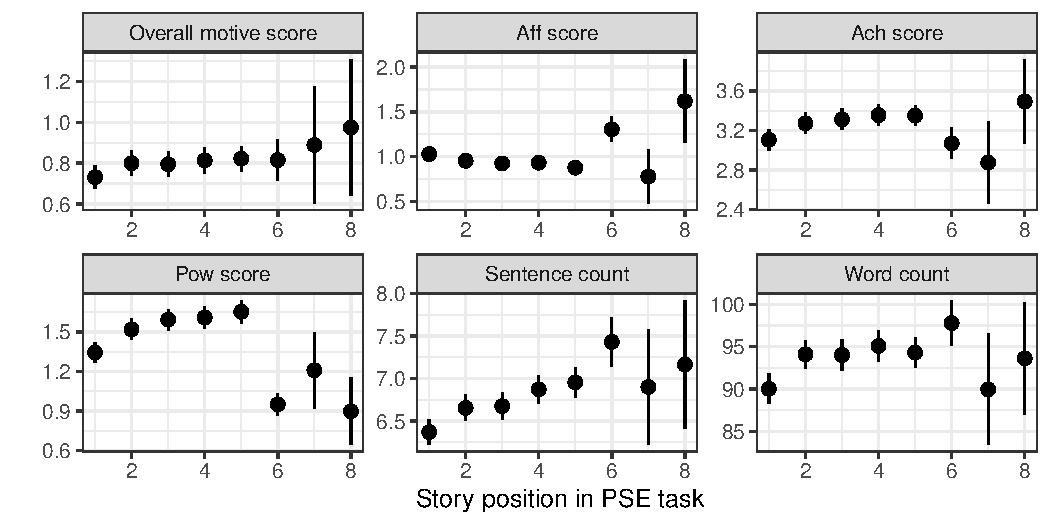
\includegraphics[width=.9\textwidth]{figure/picPosPlot-1} 

}

\caption[Descriptive motive scores, sentence count, and word count for each picture position]{Descriptive motive scores, sentence count, and word count for each picture position. Error bars are 95\% confidence intervals for the mean. Note that this descriptive plot somewhat confounds specific picture stimuli with picture position, as only some picture stimuli where located at positions 6, 7, and 8. Figure available at https://osf.io/dj8g9/, under a CC-BY4.0 license.}\label{fig:picPosPlot}
\end{figure*}


\end{knitrout}

Note that this descriptive plot to some extent confounds specific picture stimuli with picture position, as only some picture stimuli where located at positions 6, 7, and 8. For a formal test that controls for this counfound and the cross-classified data structure in general, we conducted mixed effect models with picture position as predictor, raw motive scores, sentence count, and word count as dependent variables, and random intercepts for \emph{pic\_id}, and \emph{person\_id}.\footnote{We had to remove random slopes for \emph{pic\_position} and random effects for \emph{study\_id} to achieve model convergence. Instead we added \emph{study\_id} as categorical fixed effect to control for mean level differences.} 

Also in this analysis, no consistent decrease of motive imagery for later pictures could be found. In contrast, later picture positions showed a trend towards longer stories with more motive codings, resulting in positive effects of picture position on overall motive scores ($b$ = 0.03, \emph{SE} = 0.01, \emph{p} = .011), \emph{ach} motive scores ($b$ = 0.01, \emph{SE} = 0.01, \emph{p} = .175), \emph{pow} motive scores ($b$ = 0.05, \emph{SE} = 0.01, \emph{p} < .001), sentence counts ($b$ = 0.11, \emph{SE} = 0.01, \emph{p} < .001), or word counts ($b$ = 0.79, \emph{SE} = 0.14, \emph{p} < .001). Only for \emph{aff} scores a significant but small negative effect could be found ($b$ = -0.03, \emph{SE} = 0.01, \emph{p} < .001).


\section{A Database of Pictures Used in PSEs}

All 54 pictures in the PSE database are provided in an OSF project (\url{https://osf.io/pqckn/}). This project also includes a table that shows the license and the provenance of each picture, as far as this information could be reconstructed. 

This collection of pictures includes some classic pictures (such as the ``standard six'' set, \nptextcite{schultheiss_MeasuringImplicitMotives_2007}, and some TAT pictures), but also pictures that have been added to the PSE stimulus pool more recently. As the license of some pictures is not clear, four experts (Birk Hagemeyer, Felix Schönbrodt, Lena Schiestel, and Larissa Sust) searched for 30 new pictures, all of which promised to have a considerable motive pull. All of these new pictures (starting with the label ``newpic'') have an open license (CC0, CC-BY, or CC-BY-SA) and therefore can be safely reused for research and other purposes. Figure~\ref{fig:demopic} exemplarily shows six of these new pictures, all of which had a strong overall motive pull in a preliminary dataset.


\begin{figure*}[htp]
  \begin{center}
	\includegraphics[width=\linewidth]{demopics/demopic.pdf}
  \end{center}
  \caption{Examples of new pictures with an open license. Credits: \emph{newpic04}: CC-BY, MBWA PR GmbH; \emph{newpic07}: CC-BY-SA, Idobi, via Wikimedia Commons; \emph{newpic09}: CC0; \emph{newpic10}: public domain; \emph{newpic12}: CC-BY, Pete Lewis / Department for International Development; \emph{newpic18}: CC0.}
  \label{fig:demopic}
\end{figure*}


\section{Updated Picture Norms}

Descriptive picture pull statistics have been published for the six standard pictures by \citeauthor{schultheiss_AssessmentImplicitMotives_2001} (\citeyear{schultheiss_AssessmentImplicitMotives_2001}; $n$ = 424, German stories), \citeauthor{pang_assessing_2005} (\citeyear{pang_assessing_2005}; $n$ = 320, English stories), \citeauthor{pang_ContentCodingMethods_2010} (\citeyear{pang_ContentCodingMethods_2010}; $n$ = 81, English stories), and \citeauthor{schultheiss_AreImplicitExplicit_2009} (\citeyear{schultheiss_AreImplicitExplicit_2009}; $n$ = 190, English stories). All of these norms employed the 2nd-sentence rule.

Here we present updated norms for German PSE stories, which are based on larger samples and sentence-wise coding without the 2nd-sentence rule. Sample sizes vary between pictures, depending on how often a picture has been used in the studies included in the database. Table~\ref{tab:norms} shows descriptive statistics for all pictures that had at least 50 stories, ordered by overall motive pull, which is computed as the sum of all three raw motive scores. Furthermore, we present descriptive statistics for activity inhibition, which is computed by counting the frequency of the word ``not'' in each story.\footnote{Descriptive statistics for all pictures, including the new pictures, are at \url{https://osf.io/pqckn}.}

\begin{table*}
	\begin{threeparttable}
		\caption{Means and Standard Deviations of Raw Motive Scores Across Coding Categories and Pictures.}
		\label{tab:norms}
		\tiny
		\begin{tabularx}{\textwidth}{rllllllr}
		\toprule
% latex table generated in R 3.5.2 by xtable 1.8-4 package
% Fri Sep 13 16:21:51 2019
 & Pic ID & Aff & Ach & Pow & Overall & Activity Inhib. & Word count & \emph{n} \\ 
  \hline
  1 & newpic9 & 0.77 (1.01) & \textbf{1.82} (1.27) & \textbf{2.11} (1.46) & 4.70 & 0.40 (0.70) & 84 (33) & 198 \\ 
    2 & applause & \textbf{1.88} (1.47) & 0.81 (1.12) & \textbf{1.77} (1.53) & 4.47 & 0.59 (0.91) & 90 (34) & 1195 \\ 
    3 & sorrow & \textbf{2.48} (2.03) & 0.16 (0.61) & \textbf{1.65} (1.58) & 4.28 & 1.18 (1.17) & 90 (33) & 141 \\ 
    4 & bicycle race & 0.13 (0.46) & \textbf{3.31} (1.99) & \textbf{0.80} (1.00) & 4.24 & 1.11 (1.46) & 97 (62) &  83 \\ 
    5 & beachcombers & 0.62 (1.10) & 0.14 (0.50) & \textbf{3.41} (1.87) & 4.17 & 0.75 (0.96) & 97 (34) & 797 \\ 
    6 & three people & \textbf{3.26} (1.84) & 0.02 (0.22) & 0.69 (1.02) & 3.98 & 0.89 (0.99) & 96 (28) &  81 \\ 
    7 & soccer duel & 0.13 (0.36) & \textbf{2.42} (1.63) & \textbf{1.16} (1.36) & 3.70 & 0.66 (0.89) & 86 (29) & 141 \\ 
    8 & *nightclub scene & \textbf{2.39} (1.67) & 0.14 (0.41) & \textbf{1.08} (1.25) & 3.61 & 0.57 (0.96) & 93 (37) & 2311 \\ 
    9 & burglar & \textbf{2.04} (1.76) & 0.15 (0.46) & \textbf{1.25} (1.48) & 3.44 & 0.98 (1.31) & 92 (31) & 141 \\ 
   10 & woman & \textbf{1.56} (1.62) & 0.16 (0.70) & \textbf{1.71} (1.51) & 3.44 & 0.91 (1.19) & 94 (40) & 119 \\ 
   11 & *couple by river & \textbf{3.03} (1.80) & 0.03 (0.25) & 0.34 (0.72) & 3.41 & 0.72 (1.11) & 94 (40) & 1854 \\ 
   12 & newpic10 & \textbf{1.71} (1.22) & 0.68 (1.08) & \textbf{0.92} (1.05) & 3.32 & 0.35 (0.59) & 87 (35) & 196 \\ 
   13 & kennedy nixon & 0.10 (0.38) & \textbf{1.30} (1.33) & \textbf{1.82} (1.43) & 3.22 & 0.44 (0.74) & 85 (31) & 799 \\ 
   14 & architect at desk & \textbf{2.23} (1.67) & 0.48 (0.81) & 0.49 (0.84) & 3.20 & 0.38 (0.80) & 107 (35) & 408 \\ 
   15 & *women in laboratory & 0.34 (0.77) & \textbf{1.51} (1.26) & \textbf{1.28} (1.31) & 3.13 & 0.69 (1.02) & 91 (34) & 2331 \\ 
   16 & *boxer & 0.34 (0.79) & \textbf{1.68} (1.38) & 0.81 (1.11) & 2.83 & 0.67 (1.02) & 89 (37) & 1724 \\ 
   17 & violin & \textbf{0.98} (1.12) & 0.76 (1.03) & \textbf{1.05} (1.15) & 2.79 & 1.01 (1.29) & 99 (46) & 143 \\ 
   18 & *trapeze artists & 0.73 (1.11) & \textbf{1.15} (1.14) & \textbf{0.84} (1.02) & 2.72 & 0.52 (0.87) & 91 (37) & 2316 \\ 
   19 & newpic12 & 0.55 (0.94) & 0.82 (1.11) & \textbf{1.27} (1.51) & 2.63 & 0.65 (0.95) & 83 (34) & 196 \\ 
   20 & newpic22 & 0.46 (0.81) & \textbf{1.53} (1.48) & 0.51 (0.88) & 2.50 & 0.41 (0.74) & 78 (34) & 200 \\ 
   21 & lacrosse duel & 0.20 (0.47) & \textbf{1.95} (1.36) & 0.30 (0.52) & 2.44 & 0.73 (0.98) & 92 (36) &  97 \\ 
   22 & neymar \& marcelo & 0.35 (0.79) & \textbf{1.20} (1.13) & \textbf{0.86} (1.11) & 2.41 & 0.50 (0.73) & 59 (25) & 354 \\ 
   23 & *ship captain & 0.47 (0.89) & 0.20 (0.53) & \textbf{1.56} (1.39) & 2.23 & 0.78 (1.12) & 94 (36) & 2612 \\ 
   24 & group & 0.85 (1.23) & 0.20 (0.55) & \textbf{1.13} (1.15) & 2.18 & 0.79 (1.08) & 89 (40) & 125 \\ 
   25 & newpic1 & 0.49 (0.84) & \textbf{0.85} (1.09) & \textbf{0.82} (1.03) & 2.16 & 0.98 (1.18) & 82 (35) & 202 \\ 
   26 & window & 0.94 (1.41) & 0.11 (0.34) & 0.72 (1.15) & 1.78 & 0.93 (1.05) & 90 (43) & 123 \\ 
   27 & canyon & 0.68 (0.96) & 0.19 (0.48) & 0.89 (1.27) & 1.76 & 0.59 (0.90) & 81 (44) & 111 \\ 
   28 & men on ship & 0.08 (0.35) & 0.31 (0.62) & \textbf{0.79} (0.78) & 1.18 & 0.36 (0.73) & 86 (27) &  95 \\ 
   \hline

		
		\bottomrule
		\end{tabularx}
		\begin{tablenotes}[para,flushleft]
			{\small
			\vspace*{0.75em}
			\textit{Note.} \emph{Overall} is the sum of all three motive categories (aff + ach + pow). Pictures are ordered along their overall motive pull. Bold motive scores indicate that $\geq$ 50\% of participants responded with at least one motive score to the picture. Pictures of the ``standard six'' set are marked with an asterisk. \emph{Activity Inhib.} = Activity Inhibibition. The actual pictures are provided in an OSF project (\url{https://osf.io/pqckn/}).}
	      \end{tablenotes}
	  \end{threeparttable}
\end{table*}


Pictures differ in their pull for multiple types of motive imagery. Some pictures are mostly monothematic, such as \emph{couple by river} or \emph{couple sitting opposite a woman} which almost exclusively elicit affiliation imagery. Other pictures elicit imagery from two (e.g., \emph{women in laboratory} for \emph{ach} and \emph{pow}), or three motives (e.g., \emph{applause} or \emph{trapeze artists}). The propensity of a picture to elicit imagery from multiple motives has also been termed \emph{cue ambiguity} \parencite{pang_ContentCodingMethods_2010,smith_MethodologicalConsiderationsSteps_1992,jacobs_MethodInvestigatingCue_1958}.
Figure~\ref{fig:ternary} shows a ternary plot \parencite{hamiltonGgternExtensionGgplot22017} that visualizes whether pictures are rather monothematic (located at the corners of the triangle), pull for two motives (around the midpoint of each side of the triangle), or pull for multiple motives (in the middle of the triangle).


\begin{knitrout}
\definecolor{shadecolor}{rgb}{0.969, 0.969, 0.969}\color{fgcolor}\begin{figure*}

{\centering 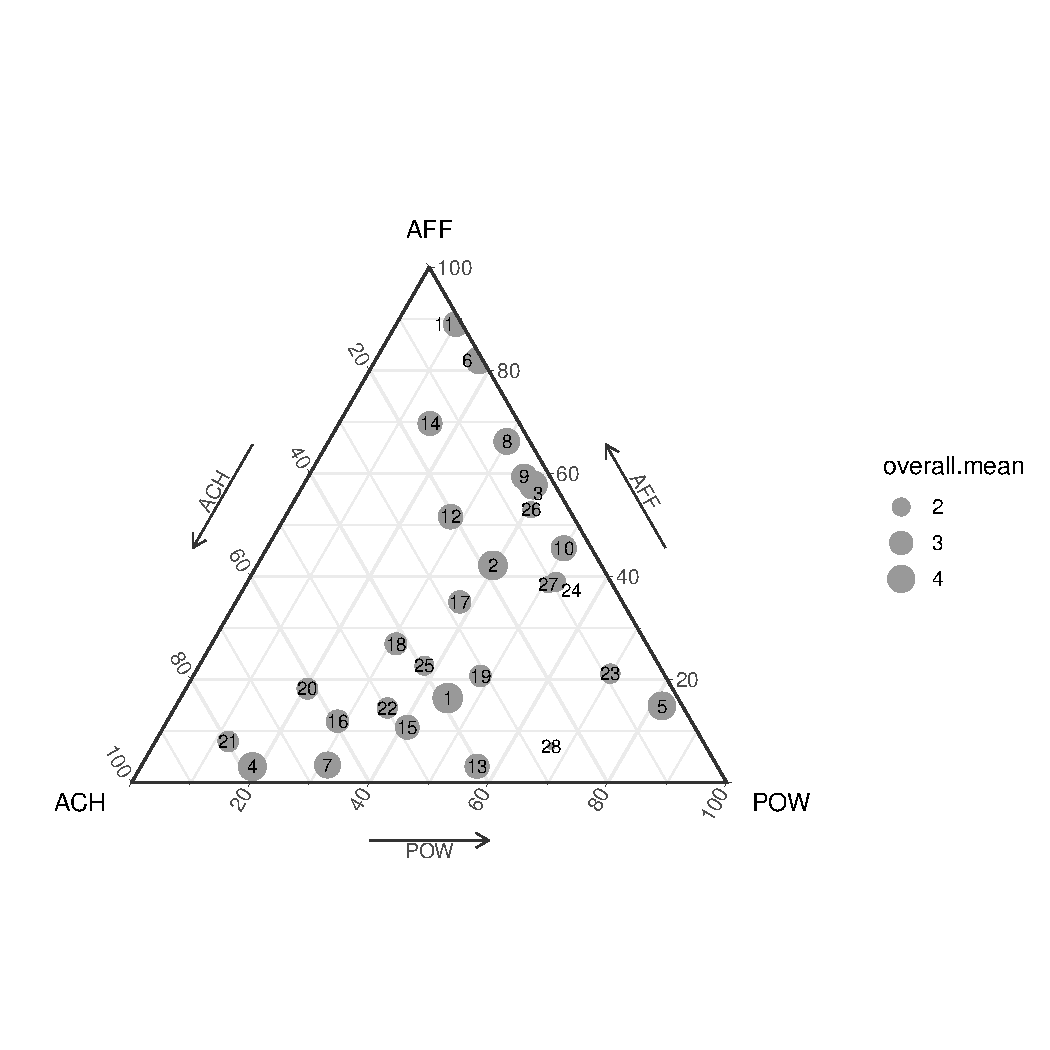
\includegraphics[width=.9\textwidth]{figure/ternary-1} 

}

\caption[Relative motive pull of pictures]{Relative motive pull of pictures. Numbers correspond to picture numbers in Table 8. Figure available at https://osf.io/dj8g9/, under a CC-BY4.0 license.}\label{fig:ternary}
\end{figure*}


\end{knitrout}

\section{Availability of the Databases}

Both the database on coded PSE stories (\url{https://osf.io/dj8g9/} and \url{https://github.com/nicebread/PSE-Database/blob/master/README.md}) and the picture database (\url{https://osf.io/pqckn/}) can be downloaded and reused freely from the Open Science Framework under a CC-BY 4.0 license. Please cite this publication if you use either database in your work.
As we expect that the PSE database will grow over time, we put a version number on it and archive old versions. We urge researchers to always refer to the specific version number when the database is used in order to ensure reproducibility.

\section{Discussion}

In this paper, we presented two databases: (a) A database of 183,408 sentences, nested in 26,389 PSE stories, provided by 4,570 participants, coded by experts using the Winter (\citeyear{winter_ManualScoringMotive_1994}) \emph{Manual for scoring motive imagery in running text}, and (b) a database of 54 classic and new pictures that have been used in PSE research. Furthermore, we provided descriptive statistics on typical sentence and word counts, as well as analyses and recommendations for how to correct motive scores for story length. Last but not least, we updated norm values for picture pulls.

We see several potential scenarios for using these databases. The primary intention for creating the PSE story database was to provide a large training dataset for automatic text analysis. We want to emphasize that these expert-coded sentences go beyond a simple sentiment analysis (e.g., positive vs. negative product reviews) that can quite easily be implemented using dictionaries \parencite[e.g.,][]{feldman_TechniquesApplicationsSentiment_2013}. In contrast, coding implicit motives requires deep semantic processing, evaluating nuances in meaning, differentiating negations, hypothetical from actual actions, questions, and much more. To what extent mathematical text models or machine learning algorithms are able to replicate human codings in the Winter coding system is an open question (see, however, \nptextcite{schultheiss_are_2013} for a potential approach to automatic coding). In addition to supervised learning that attempts to approximate human codings, the dataset can also be used to infer structures using unsupervised learning methods, such as topic models and latent dirichlet allocation \parencite{blei_LatentDirichletAllocation_2003}.

Another potential application lies in psychometric modeling. It has been argued that measurement models based on classical test theory violate assumed underlying processes in PSEs and therefore are not applicable \parencite{atkinson_studying_1981,hibbard_critique_2003,schultheiss_reliability_2008}. This large database allows testing and developing alternative measurement models that might provide more appropriate estimates of reliability and shed light on the response processes during a PSE task (see, for example, \nptextcite{tuerlinckx_measuring_2002,lang_DynamicThurstonianItem_2014,runge_ModelingMotiveActivation_2016}). We present the first large dataset that provides PSE motive codings at the sentence level, thus allowing to investigate within-story dynamics separately from between-story dynamics. This allows testing decade-old theories of motive dynamics with high statistical power. 

In a rather simple analysis we did not find consistently that later pictures elicit less motive scores. This result might seem at odds with the results of previous studies that actually did find an effect of consummatory strength, which leads to less motive expression in later pictures \parencite{tuerlinckx_measuring_2002,lang_DynamicThurstonianItem_2014}. Note, however, that these analyses tested a different model, where not the picture position per se was the predictor of motive expression. Instead the occurence of motive imagery in previous pictures was the predictor, which is assumed to decrease the probability of additional motive expressions due to satiation processes. This and other differences make the results hard to compare, and we encourage to use the current database to do a conceptual replication and extension of previous research on consummatory effects and dynamic processes of motive expression \parencite{atkinson_dynamics_1970}.

Finally, now a systematic (though indirect) investigation of differences between labs in coding style is possible. Although all labs employed the same manual, effects such as coder drift \parencite{schultheiss_MeasuringImplicitMotives_2007} can lead to an evolution of implicit coding rules that lets labs drift apart. For a more direct test of intra- and inter-lab coding agreement, future studies should give the same text material to multiple coders of several labs and assess agreement by looking at both within-lab and between-lab variability (``multi-center evaluation''; see, for example, \nptextcite{dabbs_ReliabilitySalivaryTestosterone_1995}).

The updated picture norms allow to select appropriate sets of pictures for a PSE. For example, it has been recommended to select pictures with a high motivational pull for the targeted motives \parencite{schultheiss_MeasuringImplicitMotives_2007,smith_MethodologicalConsiderationsSteps_1992}, but also some pull for other motives (``picture cue ambiguity'', \nptextcite{pang_ContentCodingMethods_2010}). Beyond ambiguity on the picture level, it has also been argued that ambiguity on the level of the picture \emph{set} is important for reliability and validity of a PSE \parencite{ramsay_SetAmbiguityKey_2013}. 

With the large collection of available pictures and their updated norms, such choices can be empirically informed. We encourage researchers who use a PSE to refer to the unique IDs of the picture database in their methods section. A common and standardized catalogue of PSE pictures enhances the replicability of studies, but also the reusability and interoperability of research results, as such clear identifiers allow the aggregation and reanalysis of datasets. 
This picture database is intended to be a ``living document'' which is constantly updated with new pictures and updated norms. Therefore we suggest that researchers who use new pictures contact the first author of this paper if they want to add a new picture to the database. (Preferably pictures with a permissive license that allows reuse.) 

An obvious limitation is that the presented databases, picture norms, and recommendations only apply to the Winter (\citeyear{winter_ManualScoringMotive_1994}) coding system, and strictly speaking only applied to PSE stories written in German. We recommend that such large data collections should also be done for other languages and other coding systems.

To conclude, we hope that these two public databases are a helpful resource both for PSE researchers and more generally for researchers interested in text content analysis, and that they refuel interest in methodological and psychometric research about measuring implicit motives with Picture Story Exercises.

\section{Author contributions}

BLINDED
% \small
% \emph{Felix Schönbrodt}: Aggregated, cleaned, preprocessed, and analyzed data; provided multiple datasets; coded stories; searched for new pictures; wrote manuscript. \emph{Birk Hagemeyer}: Provided dataset; searched for new pictures; wrote manuscript. \emph{Veronika Brandstätter}: Provided multiple datasets. \emph{Thomas Czikmantori}: Provided multiple datasets. \emph{Peter Gröpel}: Provided dataset. \emph{Marie Hennecke}: Provided multiple datasets. \emph{Laura Israel}: Provided dataset. \emph{Kevin Janson}: Provided dataset; coded stories. \emph{Nina Kemper}: Provided dataset; coded stories. \emph{Martin Köllner}: Provided multiple datasets. \emph{Philipp Kopp}: Provided dataset. \emph{Andreas Mojzisch}: Provided dataset. \emph{Raphael Müller-Hotop}: Provided dataset. \emph{Johanna Prüfer}: Provided dataset. \emph{Markus Quirin}: Provided dataset. \emph{Bettina Scheidemann}: Provided multiple datasets; coded stories. \emph{Lena Schiestel}: Provided dataset; coded stories; searched for new pictures. \emph{Stefan Schulz-Hardt}: Provided dataset. \emph{Larissa Sust}: Provided dataset; coded stories; searched for new pictures. \emph{Caroline Zygar}: Provided dataset; coded stories. \emph{Oliver Schultheiss}: Provided multiple datasets; coded stories; wrote manuscript.

All coauthors critically reviewed, commented on, and approved the final manuscript.


\printbibliography

\end{document}

% pandoc -s AMC-Database.tex -o AMC-Database.docx
